\chapter{Introdução}
\label{cap-introducao}

\section{Contexto}
\label{section:contexto}

\citeonline{indiceglobaldoempreendedorismo} afirma que menos de 1\% das empresas do Brasil conseguem manter uma taxa de crescimento acima dos 20\% anuais por um período de três anos consecutivos mas as mesmas foram responsáveis por mais de 40\% dos novos empregos gerados no país, em média elas geram cerca de 100x mais empregos do que as empresas do Brasil. Algumas dessas empresas com alto potencial de crescimento são conhecidas como startups.

\citeonline{Graham2012} afirma que o único fator essencial para que uma organização seja classificada como startup é o seu crescimento, para ele qualquer outro fator nada mais é do que um reflexo deste. Idealmente Graham defende que startups precisam crescer entre 5 e 7\% por semana e que qualquer indicador acima de 10\% seria algo excepcional. Para \citeonline{Sutton2000} a característica mais básica de uma startup é ser nova e inexperiente quando comparada com organizações estabelecidas e maduras, ele também as caracteriza como organizações que trabalham com poucos recursos e geralmente acompanham novas tendências de tecnologia e mercado, além de altamente sensíveis à diversos fatores influenciadores (investidores, clientes, parceiros e concorrentes).

Segundo \citeonline{Ries2011}, uma das principais referências acerca do tema, uma startup é uma instituição humana projetada para criar novos produtos e serviços sob condições de extrema incerteza. Para Ries o maior objetivo de uma startup é descobrir qual o produto certo que os consumidores queiram e estejam dispostos a comprar, e/ou usar, o mais rápido possível. \citeonline{isenberg2016} identificou em pesquisa que a maior parte das pessoas entrevistadas associavam o termo ``startup'' com empresas de tecnologia como o ``Snapchat'' ou o ``WhatsApp''.

\citeonline{Paternoster2014} diz que para construir produtos tecnologicamente inovadores geralmente elas precisam utilizar novas tecnologias, ferramentas e técnicas de gestão e desenvolvimento. Esse cenário condiz com o mapeamento realizado por \citeonline{Polovets2014}, o qual constatou que a maior parte das startups analisadas utilizam tecnologias como Javascript, Node.js, Ruby, Ruby on Rails, Python e HTML5 e hospedam seus softwares em grandes infraestruturas escaláveis como Amazon Web Services e Heroku. 

De volta ao Brasil, \citeonline{Brinded2015} relata que o país é o terceiro com o maior número de empreendedores do mundo, correspondendo a cerca de 13,8\% da população. Para \citeonline{Acs2016} um dos destaques do Brasil em comparação ao restante do mundo é a percepção de oportunidade.

Nessa linha, governos das três esferas brasileiras (Federal, Estaduais e Municipais) buscam desenvolver políticas públicas de fomento e suporte aos seus ecossistemas empreendedores afim de atrair investimentos, gerar empregos e aumentar a arrecadação de impostos, alguns dos exemplos de políticas públicas com foco em startups são o Inovativa Brasil, Startup Brasil, Fundo Criatec, editais de subvenção por meio de Fundações de Apoio à Pesquisa, FINEP, etc. Além disso alguns projetos de lei como a Lei da Inovação e o Marco Legal da Ciência, Tecnologia e Inovação buscam trazer flexibilidade para o ambiente regulatório do Brasil com o objetivo de aumentar as chances de sucesso e crescimento dessas empresas. Do lado privado e da sociedade civil organizada instituições como a Endeavor e a Dínamo buscam atuar de forma a apoiar governos nos processos de regulamentação e fomento aos setores empreendedores.

Trazendo para o contexto do Distrito Federal, o estado vive um dos seus momentos de maior atividade no ecossistema de startups local, embora o país e a cidade estejam passando por recessão e crises política e econômica o cenário é favorável e a realização de grandes eventos como o AgileBrazil, a World Conference on International Telecommunications, a Campus Party e diversos outros menores organizados pela comunidade local, como meetups, o evento Capital Empreendedora, o surgimento de aceleradoras locais e a movimentação das universidades são reflexo do aumento do interesse dos brasilienses em relação ao tema empreendedorismo. Também houve menção à Brasília no"Startup Awards 2017", premiação promovida pela Associação Brasileira de Startups (ABStartups) com o objetivo de identificar os maiores destaques do ano no Brasil, a universidade UniCeub está entre as indicadas para o prêmio de "Melhor Universidade" e o "Cerrado Valley" como melhor comunidade.

A baixa expectativa de concursos públicos para os próximos anos também é um fator favorável para o empreendedorismo, forçando os jovens a buscar alternativas que não a estabilidade financeira provida pelo serviço público, principal motivo para uma cultura empreendedora tão ruim na cidade, como constatado pela \citeonline{indiceglobaldoempreendedorismo}. \citeonline{Sun2011} relata que a Professora da Harvard Business School Janet. J. Kraus acredita que as crises são os melhores momentos para se iniciar um novo negócio, justamente quando os custos de oportunidade são baixos. 

\section{Justificativa}
\label{section:justificativa}

\citeonline{Paternoster2014} enfatiza que pesquisas acadêmicas são necessárias para apoiar as atividades relacionadas a startups e guiar as ações de diversos atores que compõem um ecossistema, como empreendedores, agentes públicos, investidores e acadêmicos.

Com base em uma análise das principais publicações acerca do tema nos últimos 300 anos \citeonline{Filion1998} divide o progresso dos estudos acerca do empreendedorismo em cinco períodos representados pela Tabela \ref{table:tendencias_nas_publicacoes_acerca_do_empreendedorismo}.

\begin{table}[!htb]
	\centering
	\begin{tabular}{ | p{6cm} | p{6cm} | p{3cm} | }
		\hline
		Tema & Perspectiva & Período \\ \hline
		O que fazem os empreendedores & Econômica & 1700 - 1950 \\ \hline
		Quem são os empreendedores & Comportamental & 1960 - 1980 \\ \hline
		O que fazem os empreendedores & Administrativa(finanças, marketing, operações, recursos humanos) & 1980 - Atual \\ \hline
		Quais tipos de suporte são necessários para empreendedores & Ciências Sociais(incluindo economia, geográfia e sociologia) & 1985 - Atual \\ \hline
		O que são atividades empreendedoras e quais Competências são necessárias & Empreendedorismo & 1990 - Atual \\ \hline
	\end{tabular}
	\caption{Tendências nas publicações acerca do Empreendedorismo}
	\label{table:tendencias_nas_publicacoes_acerca_do_empreendedorismo}
\end{table}

Embora Filion tenha relatado que até meados da década de 90 pouco se explorou sobre ecossistemas empreendedores \citeonline{Cukier2016}  demonstrou que nos últimos sete anos houve um crescimento superior a 1000\% na quantidade de artigos acadêmicos indexados pela plataforma Google Scholar com o termo ``Startup Ecosystems'', resultado explicitado na Figura \ref{figure:papers_about_startup_ecosystems}.

\begin{figure}[!htb]
	\centering
	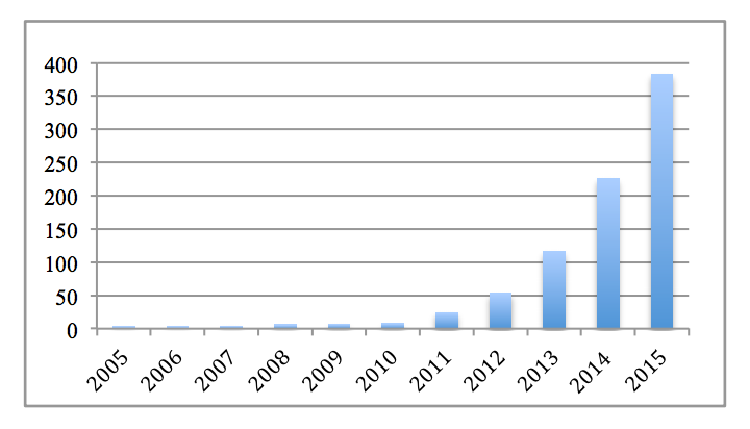
\includegraphics[width=11cm,angle=0]{figuras/papers_about_startup_ecosystems}
	\caption{Frequência do termo ``Startup Ecosystem'' no Google Scholar}
	\label{figure:papers_about_startup_ecosystems}
\end{figure}

O crescimento pela demanda por estudos sobre ecossistemas de startups também foi identificada por \citeonline{Unterkalmsteiner2016}, os mesmos enfatizam a importância de pesquisas que busquem responder questões que envolvam os elementos chaves de um ecossistema frutífero, os tipos de ecossistemas, como eles evoluem e técnicas de avaliação e mensuração de qualidade. \citeonline{Lemos2011} enfatiza que faltam teorias consolidadas sobre as relações entre os diversos elementos que compõem um ecossistema.

Portanto, nota-se que é crescente a demanda por estudos sobre ecossistemas de startups e como os diversos fatores que os compõem interagem entre si e impactam o seu desenvolvimento. Até o momento há poucos dados e estudos disponíveis sobre o setor e no atual momento do ecossistema de startup do Distrito Federal é de extrema relevância que sejam estudados sua maturidade, a relação entre seus atores, quem são os empreendedores, onde estão e quais os seus desafios, quais os pontos fortes e os pontos de melhora do ecossistema, etc. para que os atores engajados em fomentar o ecossistema (empreendedores, sociedade civil organizada, entidades representativas, academia, governo, etc.) possuam insumos para suas tomadas de decisão. 

\section{Objetivo Geral}
\label{section:objetivo_geral}

Para cumprir esse objetivo foi utilizada a metodologia de avaliação de ecossistemas de startups de tecnologia criada por \citeonline{Kon2014}, como insumo de informações foram realizadas entrevistas com atores do ecossistema em estudo e análises de dados e pesquisas disponíveis no contexto do DF. Mais detalhes sobre a metodologia são explorados no capítulo \ref{cap-metodologia} e os resultados nos capítulos seguintes.

\section{Objetivos Específicos}
\label{section:objetivos_especificos}

Este trabalho consiste em um estudo de caráter exploratório do ecossistema de startups de tecnologia do Distrito Federal com o objetivo específico de explora-lo para que seja feita uma avaliação do seu atual momento e sua maturidade. Como resultado final é esperado uma síntese dos dados coletados de forma a gerar uma visão generalista de algumas das características como pontos fortes e pontos de melhora do ecossistema local de acordo com a visão dos atores que o compõem. 

\section{Organização do Trabalho}
\label{section:organizacao_do_trabalho}

Este Trabalho de Conclusão de Curso em mãos está organizado em quatro capítulos: primeiramente uma breve introdução com o contexto o qual está inserido e os objetivos de pesquisa.

O Capítulo \ref{cap-sobre-a-proposta-e-a-metodologia} explora o cenário de pesquisa em torno de ecossistemas de startups, o capítulo \ref{cap-metodologia} descreve a metodologia que será aplicada em Brasília, principalmente no que tange os indicadores utilizados para mensurar sua maturidade.

O Capítulo \ref{cap-resultados} apresenta os resultados obtidos, o que fora descoberto, qual a visão dos empreendedores entrevistados e quais ações podem ser tomadas para que o ecossistema do Distrito Federal evolua. Por fim, no Capítulo \ref{cap-conclusoes} é feito um apanhado de tudo o que foi explorado nos capítulos anteriores e o que fora aprendido com o desenvolvimento deste trabalho. Em seguida são apresentados os Anexos e Apêndices do trabalho.
